\chapter{Introduction}

\tododone{Introduction}

%%%%%%%%%%%%%%%%%%%%%%%%%%%%%%%%%%%%%%%%%%%%%%%%%%%%%%%%%%%%%%%%%%%%%%%

Kepler is a space observatory launched by NASA in 2009 to discover Eath-sized exoplanets orbiting other stars  \cite{2010ApJ...713L..87J}. Kepler mission developed several decades to answer the centuries-old question: How frequent are other Earth-like planets in Milkyway galaxy? In particular, what is the frequency of Earth-size planets in the Habitable-Zone of solar-like stars? There are three different types of exoplanets are common in our universe: gas giants, hot-super-Earths in short period orbits, and ice giants. The challenge is to find the terrestrial planets that are in the habitable zone of their host stars where liquid water might exist on the surface of the planet.

The scientific objective of the Kepler mission is to explore the structure and diversity of planetary systems. This mission surveys a large sample of stars to determine the percentage of terrestrial and large planets that are in or near the habitable zone of a wide variety of stars and determine the distribution of size and shapes of the orbits of these planets. Kepler mission also estimates how many planets are in multiple-star systems. After collecting a large number of data points, using many techniques scientists determine the properties of those stars that harbor planarity systems including the planets itself. 

After preprocessing raw data, the goal is to classify each detection into one of the three different categories: Planetary Candidate (PC), Astrophysical False Positive (AFP) and None transiting phenomena (NTP ). Historically this process is done by researchers looking at each observation. This is a very slow and time consuming process. During this project, I am attempting to automate this classification process using machine learning algorithms.

\section{Search for Earth-Like Planets}
\tododone{What Problem we are solving - Project Origin, Background problem domain}
\tododone{- define the problem : explain in detail about the exoplanets}
One of the most fundamental and intriguing philosophical questions has remained for at least 2300 years is whether life exists outside of our Solar System. With the science and technology has grown exponentially within the last couple of hundred years, it is now, we have the theoretical knowledge, practical and feasibility to seek answers to this question from a scientific perspective. NASA's Navigator Program is the long term project that over-seeing the missions related to  detecting and characterization of Earth-like planets. These missions consist of multidisciplinary suite of research efforts, centering on finding exoplanets that could harbor biological activity similar to terrestrial life.

In the process of searching for Earth-like planets, we will encounter a spectrum of planets. The planetary population conceivably outnumbers stellar population since a star could host many planets such as our solar system. Unlike stars\footnote{Vogt-Russell theorem states that the properties of a star are fully determined by the mass and chemical composision.}, planets can have many different characteristics, careful examination of the planets in our solar system show us that full understanding of planets, in general, requires a working knowledge of diverse fields including star formarion, orbital mechanics, geology, grophysics, climatology, agronomy, chemistry, biology and various engineering disciplines. 

we need to address a couple of questions in the search for habitable worlds:

\begin{itemize}
	\item How do planetary systems form and evolve?
	\item Are there other planetary systems like our own?
	\item Is there life elsewhere in the Universe?
\end{itemize}

Search for habitable planets begins with an understanding of the formation of planetary systems in protoplanetary disks to learn how planetary systems form, around which types of stars planets form, how often planets form, and how the disk properties effect the distribution of final planets sizes and orbits\cite{2002ApJ...580..494Y}.The primary mission for observing the formation of planetary systems will be the James Webb Space Telescope (JWST) \cite{Gardner2006}. JWST will allow us to study the earliest moments of star and planet formation. 

In the quest of finding an extraterrestrial life form, the current observations suggest that Earth-sized rocky planets may be common; however, their abundance is quite uncertain. Kepler is a one the space-based mission\cite{2010ApJ...713L..87J} that is under NASA's navigator program which observes planetary systems in our solar neighborhood. Kepler also finds correlations between the presence of Eath-like planets and both stellar characteristics and the presence and orbits of giant planets. It is important to understand that no single instrument or technique is capable of finding all planetary system components around stars of all ages. Many space and ground bases missions will use complementary instrumentations and techniques to explore majority of planetary discoveries. There are four fundamental techniques will be used to determine the architecture of planetary systems: (i) \emph{Radial Velocity Measurements} (ii) \emph{Transit Observations}, (iii) \emph{Astrometry} (iv) \emph{Direct Detection}.

To answer the question ``Is there life elsewhere in the universe?'', we need to look for habitable planets. For us to determine whether a planet is habitable, we must build observations capable of directly detecting the light from the planet, with the planet illuminated by the light from its parent star. Direct detection of these planets is an enormous technical challenge. Another way to infer habitability of a planet is to check if the planet is located in the \emph{Habitable Zoned} of the host star. Habitable Zone is the range in the distance from a star where liquid water could exist on the surface of a planet orbiting a star that possibly supports life. Liquid water is essential to all life on Earth, and so the definition of a habitable zone is based on the hypothesis that extraterrestrial life would share this requirement \cite{2014ApJ...787L..29K}. This is a very traditional definition, as a planet surface temperature may depend on other factors such as greenhouse gas abundance, its reflectivity, atmospheric and oceanic circulation, radioactive decay, and tidal heating within the planet. These energy sources can be easily allowed the planet to have subsurface liquid water reservoirs.  Jupiter's moon Europa has liquid water ocean tens of kilometers below its surface that may well be habitable for some organisms. More than 20 planets, including the nearest extrasolar planet, Proxima Centauri b \cite{2016Natur.536..437A}, have been found that are both roughly Earth-sized and orbiting within a Habitable Zoned of their stars. 


\begin{figure}[!h]
\begin{center}
        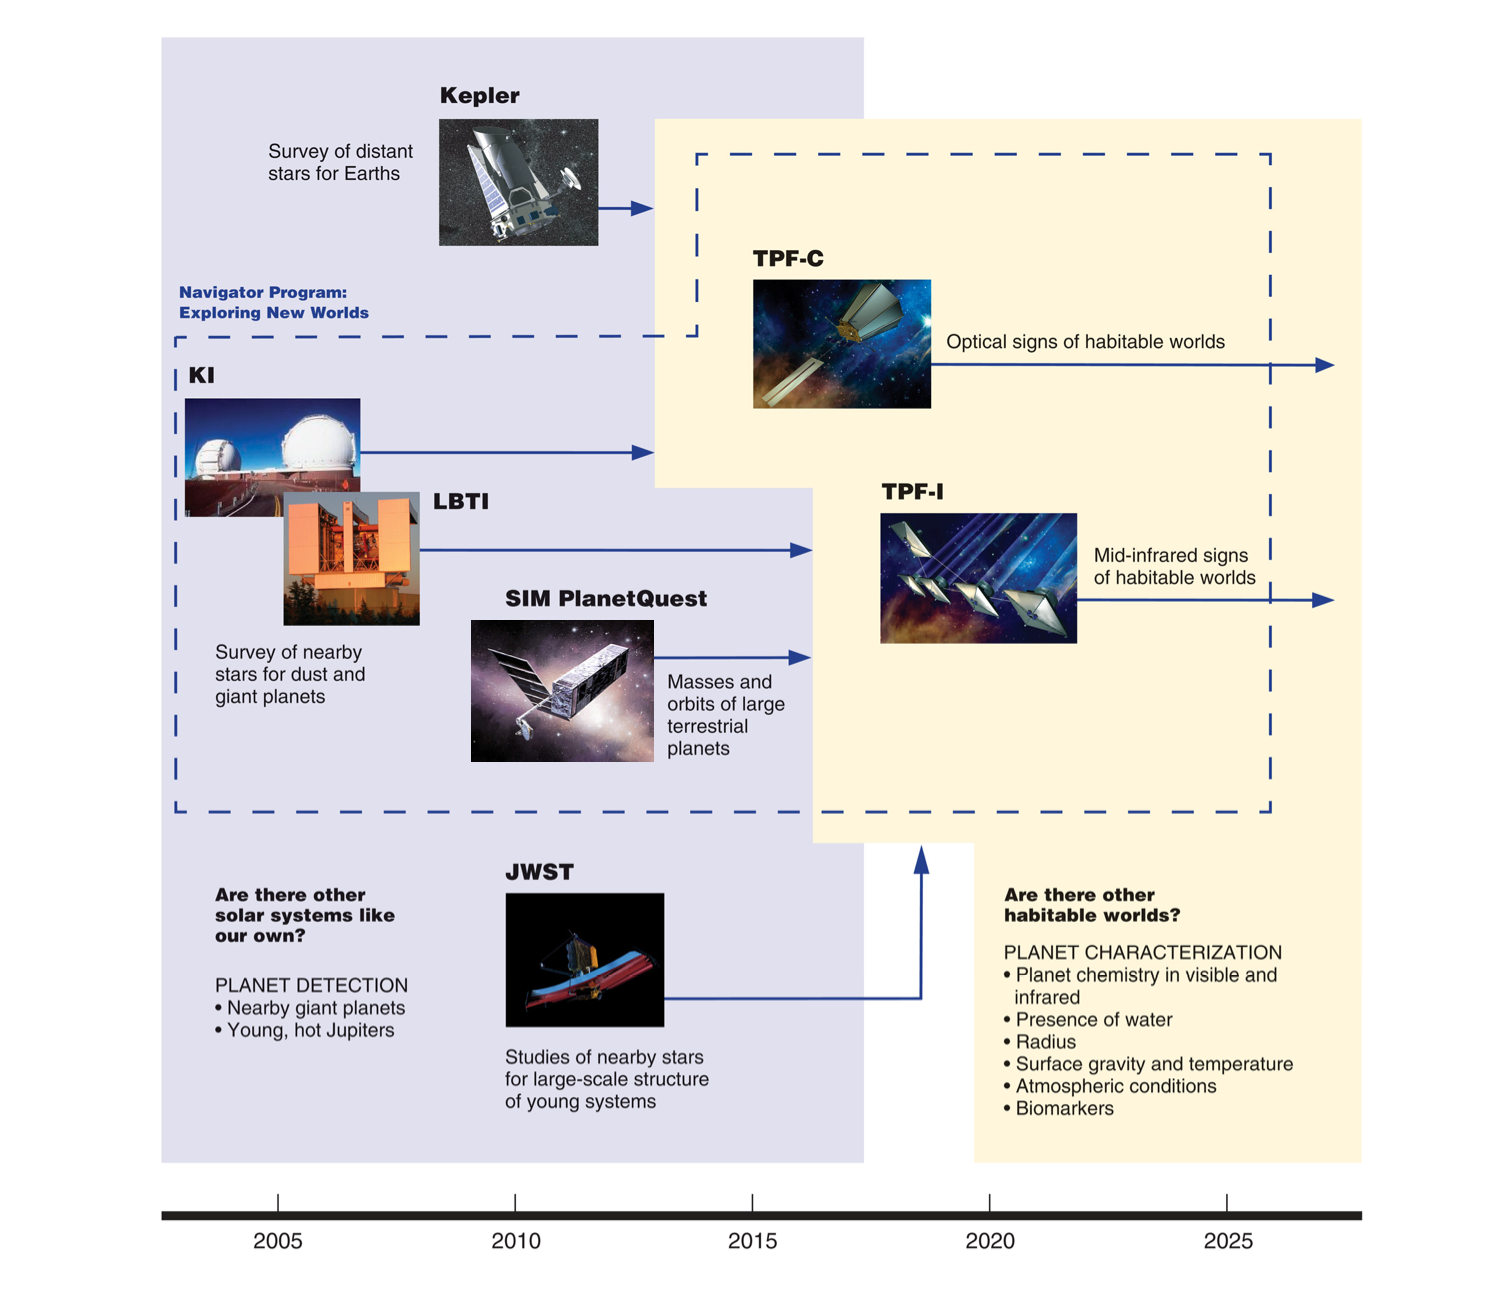
\includegraphics[width=0.8\textheight]{img/navigatorprogram.png}
        \caption{Navigator Program. National timeline including the flow of science between missions, including the \emph{Kepler} Discovery mission and JWST.
\emph{Image Credit}: NASA}  \label{fig:np}
\end{center}
\end{figure}

NASA's navigator program is a scientific program whose primary goal are to detect and characterize Earth-like exoplanets and understand the formation, and distribution of planetary systems in our Galaxy. Key features of the navigator program includes, integration of space and ground activities into a cohesive effort to find and characterize the planetary systems in our solar neighborhood. Multi-project approach to managing risk across the Navigator program by identifying the scientific and technological dependecies across the program and developing alternatives and descope to provide robustness and flexibility. The relationship between the different missions is illustrated in figure \ref{fig:np} 


\section{Kepler Mission}

Kepler mission and the spacecraft was named after one of history's revolutionary German astronomer and mathematician, Johannes Kepler\cite{voelkel2001johannes}. Kepler space observatory was launched in March of 2009 into an Earth-trailing heliocentric orbit from Cape Canaveral Air Forced Station, Florida using Delta II rocket. Spacecraft design to observe fixed field of view for an extended period. Original mission duration was planned for 3.5 years; however, the mission elapsed 7 years and 11 months. On June 19, 2009, the spacecraft sent its first science data to Earth. Spacecraft continually collect science data downlink back to Earth per month. Each dataset roughly 12 gigabytes in size. On July 14, 2012, one reaction wheel (out of four) use for pointing of the spacecraft failed; however, the spacecraft only require three wheels to operate accurately. Spacecraft continually collected data from the original field of view until a second reaction wheel failed on May 11, 2013. This ends the Kepler's primary mission. At this point spacecraft no longer point to its original field of view, and this led to the "K2" follow-on mission \cite{2014PASP..126..398H} observing different fields near the elliptic orbit. 

\section{Photometry}

The most basic information we can measure about celestial objects is the amount of energy that coming from it in the form of electromagnetic radiation. This quantity is known as flux. The science of measuring the flux from a celestial object is called Photometry. The photometer is an instrument that use to measure light intensity coming from an object. A Charge Coupled Devices (CCD) camera is essentially a grid of photometers that record and measure photons are coming from the sources that are in its field of view. The primary instrument of the Kepler spacecraft is a CCD photometer\cite{2012PASP..124.1073P}. This CCD has 0.95-meter aperture and a 105 square degree field of view (FOV).  This instrument has the sensitivity to detect Earth-like planet transit that host by a solar-like star in 6.5 hours of integration. 

\begin{figure}[!h]
\begin{center}
        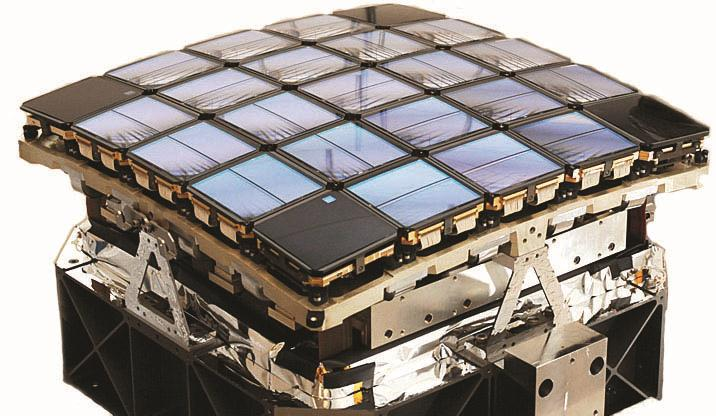
\includegraphics[width=0.3\textheight]{img/kccd.png}
	\caption{The focal plane consists of an array of 42 CCDs. Each CCD is 2.8 by 3.0 cm with 1024 by 1100 pixels. The entire focal plane contains 95 mega pixels.
mage Credits: NASA Ames and Ball Aerospace} \label{fig:kccd}
\end{center}
\end{figure}

\section{The Transit Method of Detecting Extrasolar Planets}

The Kepler spacecraft detects exoplanets using transit photometry \cite{2000ApJ...529L..45C}. If a planet orbiting a star on the plain of view and when the it moves between the detector and the star, the light that is coming from the star partially get blocked. This event is called a ``{\emph {transit}}''. For example, we can observe an occasional Venus or Mercury transit from Earth as a small black dot creeping across the Sun. During a transit, the flux we receive from the star reduce due to the transiting planet. When this happen, we say the planet transit the star, and can be detected using transit photometry. During these events, Kepler CCD collects raw data form of a sequence of stellar images, which are processed into "light-curves" tracking the brightness of a star over time. Light-curves are graphs that show the intensity of the light that observes from the star on the y-axis and the observation time on the x-axis (Figure \ref{fig:transit}). These transit data are rich with information about the planet-stellar system. The depth of the dip in the light curve and the size of the star together can be use to measure the size or the radius of the planet. The orbital period of the planet can be determined by measuring the time different between transits. Once the orbital period of the planets is known, Kepler's Third Low of planetary motion can be use to determine the average distance of the planet from its hosting star.

\begin{figure}[!h]
\begin{center}
        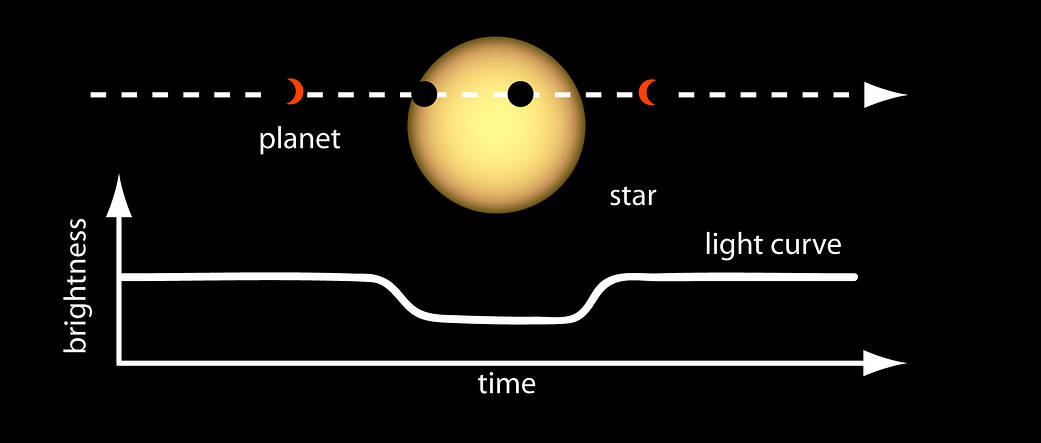
\includegraphics[width=0.7\textheight]{img/lightcurve.jpg}
        \caption{Light Curve of a Planet Transiting Its Star. Image Credit: NASA}  \label{fig:transit}
\end{center}
\end{figure}

\begin{figure}[!h]
\begin{center}
        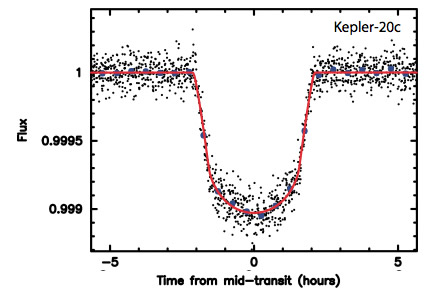
\includegraphics[width=0.6\textheight]{img/k20c.jpg}
        \caption{The light curve shown here was made from brightness data gathered by the Kepler Mission for discovery of planet Kepler-20c.
Image Credit: NASA}  \label{fig:lightcurve}
\end{center}
\end{figure}

Figure \ref{fig:lightcurve} shows the light curve made from the brightness data from Kepler Mission for the discovery of a planet named \emph{Kepler-20c}. Data clearly show the flux of the host star drop notability when the planet is in transit. This is the primary signature we are looking in the transit photometry to discover planets that are in orbits around stars. These planets create this photometric signature periodically while they are orbiting around the star. To make things more complicated, the light curves of some other objects also create similar photometric signatures: eclipsing binaries stars, certain other variable stars. During the classification stage, we need to classify these object as false positives. 


\section{Kepler Field of View (FOV)}
When it comes to where to look for exoplanets, there is a vast area in the sky we could point the spacecraft; however, there are a couple of technical requirements need to satisfy for the spacecraft to collect accurate data. The primary requirement is the field of view is always clear of the Sun and the Moon. This is preventing the Sunlight enter int to the CCD array. Kepler points away from the ecliptic, the line in the sky where the Sun, Moon, and the solar system planets traverse. Additionally, Kepler chose to look at an arm of the Milky Way galaxy that has stars similar in age and composition to our Sun and have the largest possible number of stars. The field of view region the Kepler mission is in the constellations Cygnus and Lyra, north of the visible band of the Milky Way. Figure \ref{fig:FOV2} show the Field of View superimposed over Milky Way Galaxy, Figure \ref{fig:FOV1} show the FOV relative to our Sun, Figure \ref{fig:FOV3} show the FOV relative to Cygnus. 
\begin{figure}[!h]
\begin{center}
        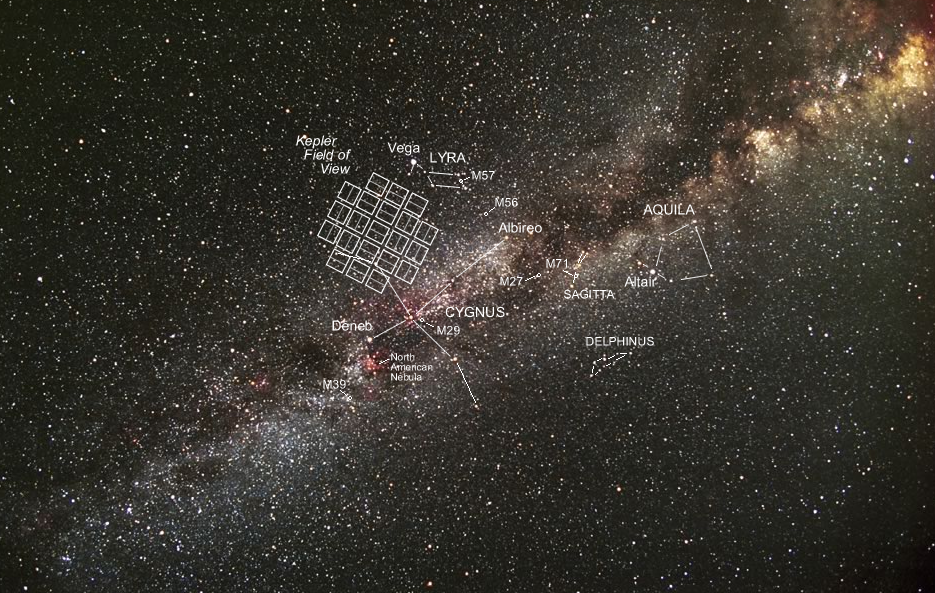
\includegraphics[width=0.55\textheight]{img/FOV2.png}
        \caption{The Kepler field of view superimposed over a photograph of the Milky Way Galaxy}  \label{fig:FOV2}
\end{center}
\end{figure}
\begin{figure}[!htb]
\minipage{0.47\textwidth}
  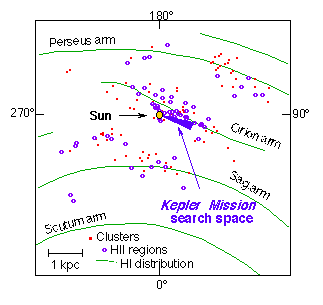
\includegraphics[width=\linewidth]{img/FOV1.png}
  \caption{Kepler FOV in extended solar neighborhood}\label{fig:FOV1}
\endminipage\hfill
\minipage{0.5\textwidth}
  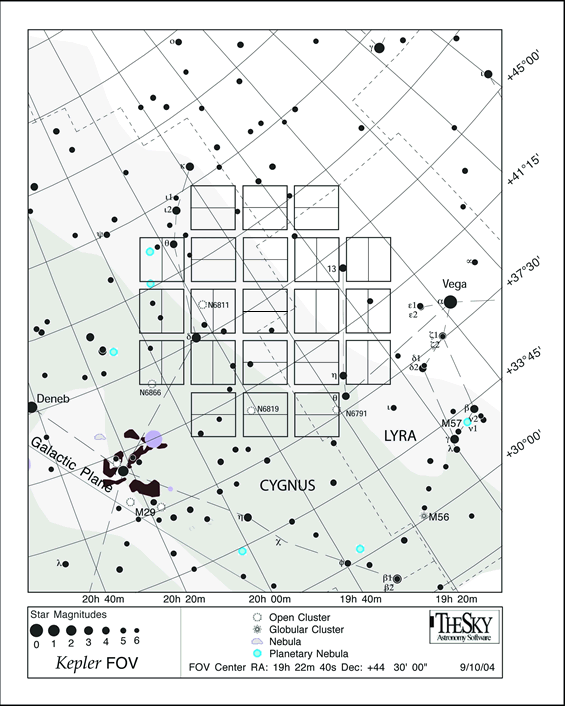
\includegraphics[width=\linewidth]{img/FOV3.png}
  \caption{Squares are 21 CCD modules.}\label{fig:FOV3}
\endminipage
\end{figure}

%\section{Kepler Data Pipleline}

\section{Kepler Pipeline}

The Kepler Pipeline \cite{2010ApJ...713L..87J} is a data reduction pipeline used for translating the Kepler raw pixel data into possible transiting planet detections. Kepler mission perform photometric observations of carefully selected stars (around 156,000) using its 115 deg$^2$ field of view (FOV) as reviewed in Borucki et el. (2010) \cite{Borucki977}
 and Koch et al. (2010)  \cite{2010ApJ...713L..79K}. The Kepler Mission Science Operations Center (SOC) at NASA Ames Research Center performs major functions on these datasets including calibrate CCD array, download data (light curves) from the spacecraft periodically, remove systematic noise \cite{2012PASP..124.1000S} and perform statistical tests to reject false positives and establish accurate statistical confidence in each detection.

\begin{figure}[!h]
\begin{center}
        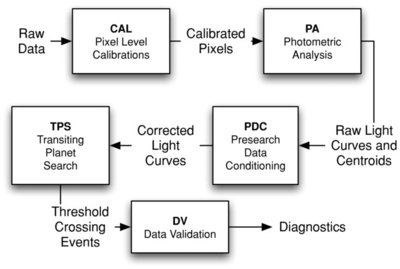
\includegraphics[width=0.5\textheight]{img/kpipeline.jpg}
        \caption{Data flow diagram for the SOC Science Pipeline. Image Credit: The American Astronomical Society}  \label{fig:kpipleline}
\end{center}
\end{figure}

Figure \ref{fig:kpipleline} show the major steps and modules of the pipeline. In particular the last two modules of the pipeline; those that identify as Threshold Crossing Events (TCEs) and their subsequent transit model fiting. TCE is a sequence of significant, periodic, planet transit-like features in the light curve of a target star. Transiting Planet Search module takes systematic error-correlated light curve for a star and seach parameter space for possible transit signatures. This module outputs a TCE or say that does not exists TCE event on the target star. This produce smaller subset of target stars what is given to the Data Validation (DV) module. DV module takes initial TCE and gaps the transit signatures from the light curve and uses the Transiting Planet Search to find additional TCEs on the same target star. This process repeats until it finds all the TCEs on given star. More details on this process explained by Mandel and Agol (2002) \cite{2002ApJ...580L.171M} and Claret and Bloemen (2011) \cite{2011yCat..35290075C}.

TPS algorithm detects transit-like features in light curves by applying noise compensating, wavelet-based matched filtering. TPS characterized the power spectral density (PSD) of the observation noise as a function of time to implement a whitening filter in the wavelet domain. The trial transit pulse is whitened and correlated against the whitened flux time series. Features with correlations above the threshold of 7.1$\sigma$ are flagged as potential threshold crossing events and subjected to additional tests in TPS to guard against false alarms.

Algorithm searches a parameter space with varying transit durations $D$ and produce a Single Event Statistics (SES) time series that is the significance of the detection of the reference transmit pulse centered at that particular time for each $D$

\begin{equation}\label{eq:ses}
	SES(t) = N(t) /\sqrt{D(t)}
\end{equation}

$\sqrt{D(t)}$, is the expected signal to noise ratio of a signal that exactly matches the template pulse and $N(t)$ is the correlated time series.



Multiple Event statistics (MES) is constructed that characterizes a significant detection in a search over varying orbital period $p$ and epochs (phase) $t_0$ by folding $N(n)$ and $D(n)$. MES  $>$ 7.1$\sigma$ may produce a TCE if it also passes additional statistical tests. SES and MES are the basis of some of the attributes used in the training set.


\section{KOI and TCE Attributes }

The Threshold Crossing Events (TCE) catalog contain a sequence of transit-like features in the flux time series of a given target star. These TCE data can download from NASA Exoplanet Archive databases \footnote{\url{http://exoplanetarchive.ipac.caltech.edu/cgi-bin/TblView/nph-tblView?app=ExoTbls&config=q1_q17_dr24_tce}}, and also the detail description of the table fields \footnote{\url{http://exoplanetarchive.ipac.caltech.edu/docs/API_tce_columns.html }} are listed as public data. Kepler Object of Interest (KOI) catalog contains object data including many attributes. The detail attributes are listed on NASA Exoplanet Archive website \footnote{\url{
http://exoplanetarchive.ipac.caltech.edu/docs/API_kepcandidate_columns.html}}, and dataset can be download from the arcive tables \footnote{\url{http://exoplanetarchive.ipac.caltech.edu/cgi-bin/TblView/nph-tblView?app=ExoTbls&config=cumulative}}. All these data cab be download as bulk using data tools available in the archive website.

%\section{Some Important Attributes}
%\label{label:important_attributes}
%There are a large number of attributes available in the KOI and TCE datasets. Out of these attributes, following attributes has significant importance in classification process according to the literature. We will be including these attributes along side with other attributes that will be determined by using Independent Component Analysis.

%\begin{itemize}
%	\item $MES_{max}$/$MES_{min}$
%	\item SNR (for all-transit model fit)
%	\item MES scaled by SES auto-correlation statistics
%	\item $\chi^{2}$ statistics for the all-transits model fit
%	\item Ratio of the planet's semi-major axis to stellar radious
%	\item The proportion of the light curve that was missing during this TCEs transit
%\end{itemize}

\section{TCE Classification Labels}

Each Threshold Crossing Event (TCE) is subject to a vetting process performed by the Kepler TCE Review Team (TCERT). During the triage (Initial) vetting stage, all TCEs are partition into two different sets: Problematic Ligh Curves that has instrumental noise and Kepler Object of Interest. KOI is a TCE that contains convincing transit-like features that do not present obvious evidence that the TCE was generated from non-transiting phenomena such as instrumental noise. These KOIs moves to next level of the vetting process performed by individuals manually inspecting light curves using detection statistics. Any indication they see the signal came from an eclipsing binary star or more complex forms of instrumental noise removed from the list. TCEs that survive this removal process are classified as Planet Candidates (PC).


We can identify three different types of classification labels in the processed dataset: Planetary Candidates (PC), Astrophysical False Positives (AFP) and non-transiting phenomena (NTP). PCs are confirmed as planets, statistically validated as planets or determined to be a planet candidate by the TCERT. AFPs are those TCEs that have been shown to be eclipsing binary stars or have shown evidence that the transiting object being detected is not located around the target tart. NTP are those TCEs that failed the initial vetting process.

%I am planning to use machine learning algorithm (Neural Network) to find a function that maps attributes produced by the Kepler Pipeline for each TCE to a classification label of PC, AFP or NTP. This classification funtion is purely based on the statistical distributions of the attributes for each TCE and the algorithm does not attempt to physically model the process of the planet transit beyond what is already present in the TCE attribute catalogs.


% \todo{Define the Problem we are solving - Classify the TCE catalog is the probme we are trying to solve}
\section{The Problem statement}

Kepler is a single instrument spacecraft that collect most contiguous and long-running photometric time series possible. Kepler observe approximately 170,000 stars simultaneously while it is operating. The fundamental objective of the Kepler mission is to detect a large number of transiting exoplanets. The ultimate goal of the primary mission was a characterize the frequency of exoplanets on diameter, orbital period and host star.  The Manual classification of the findings of Kepler object has proven very time-consuming. The new space-based, transit photometry missions such as K2 \cite{2014PASP..126..398H}, TESS \cite{2014SPIE.9143E..20R}, and PLATO 2.0 \cite{2014ExA....38..249R} also produce a large number of the dataset that demands some level of automation to do the classification. 

Using machine learning classification techniques, we can speed up the process and provide a more continuous rating of planarity candidates. There are various of machine learning classification techniques has been applied to Kepler dataset including random forests, SVM, K-mean clustering \cite{2015ApJ...800...99T, 2015ApJ...806....6M}.  In this project, we are attempting to train a Multilayered Neural Network to identify the potential planetary candidates in the Kepler dataset. 


\section{Solution Statement}

Machine learning techniques contribute a way to automate some step of exoplanet discovery. The TCE vetting process is a tedious and time-consuming (mostly a manual) process. Modern astronomical observational instruments generate a large amount of data within a short period of observational time. These observations may contain such a crucial events that need future follow-up observations using other telescopes (using other wavelengths); hence, processing these time series data and extracting meaningful information is a time sensitive process. Solution to this is to process Kepler data using machine learning algorithms to express the classification while reducing human errors. I am attempting to trained Neural Network to process the TCE catalog to automate the classification process. 


% - Explain the light curves - DONE 
% - Explain basic structure and some info about the spacecraft - DONE
% - Include some images of the field of view and spacecraft  - DONE
% \todo{Transit method - This is already Done}
% \todo{Kepler data pipeline - this is already done}
% \todo{Define the Problem we are solving - Classify the TCE catalog is the probme we are trying to solve} - DONE
% \todo{Stratergy to solve the problem - Use neural network} - Done
% \todo{Matrix that will be using - Loss function (explain the negative log likelyhood) and the confution matrix}